%! Author = elias
%! Date = 2/5/23

% Preamble
\documentclass[aspectratio=169]{beamer}

% Packages
\usepackage{amsmath}
\usepackage[utf8]{inputenc}
\usepackage{blkarray}
\usepackage{pgfplots}
\usepackage{tikz}
\usepackage{siunitx}
\usepackage{color}
\usepackage{graphicx}

\usepgfplotslibrary{units} % Allows to enter the units nicely
\pgfplotsset{compat=1.18}

\usetheme{Madrid}
\usecolortheme{beaver}

\newcommand{\FlightPathX}[1][1]{
	\begin{tikzpicture} [scale = #1]
		\begin{axis} [
				xmin = 0, xmax = 0.7,
				ymin = -3, ymax= 3,
				grid=major, % Display a grid
				grid style={dashed, red!30},
				xlabel=Zeit,
				ylabel=Position,
				x unit=\si{\second}, % Set the respective units
				y unit=\si{\meter},
			]

			\addplot[
				domain = 0:0.7,
				smooth,
				ultra thick,
				gray!50
			] {2.626712480 * x + -2.005835704};

			\addplot[
				domain = 0:0.7,
				smooth,
				only marks,
				red,
			] file[skip first] {../resources/FlightPathX.dat};


		\end{axis}
	\end{tikzpicture}
}

\newcommand{\FlightPathY}[1][1] {
	\begin{tikzpicture} [scale = #1]
		\begin{axis} [
				xmin = 0, xmax = 0.7,
				ymin = -3, ymax = 3,
				grid=major, % Display a grid
				grid style={dashed, green!30},
				xlabel=Zeit,
				ylabel=Position,
				x unit=\si{\second}, % Set the respective units
				y unit=\si{\meter},
			]

			\addplot[
				domain = 0:0.7,
				smooth,
				ultra thick,
				gray!50
			] {-0.019158488 * x + 0.029724438};

			\addplot[
				domain = 0:0.7,
				smooth,
				only marks,
				green,
			] file[skip first] {../resources/FlightPathY.dat};


		\end{axis}
	\end{tikzpicture}
}

\newcommand{\FlightPathZ}[1][1] {
	\begin{tikzpicture} [scale = #1]
		\begin{axis} [
				xmin = 0, xmax = 0.7,
				grid=major, % Display a grid
				grid style={dashed, blue!30},
				xlabel=Zeit,
				ylabel=Höhe,
				x unit=\si{\second}, % Set the respective units
				y unit=\si{\meter},
			]

			\addplot[
				domain = 0:0.7,
				smooth,
				ultra thick,
				gray!50
			] {-5.170016538 * x * x + 3.026370508 * x + 0.539997655};

			\addplot[
				domain = 0:0.7,
				smooth,
				only marks,
				blue,
			] file[skip first] {../resources/FlightPathZ.dat};


		\end{axis}
	\end{tikzpicture}
}


\newcommand{\FlightPath}[1][1] {
	\begin{tikzpicture} [scale = #1]
		\begin{axis}
			[   view={-60}{30},
				xmin=-2.1,xmax=0,
				ymin=-1,ymax=1,
				zmin=0, zmax=1,
				grid=major, % Display a grid
				grid style={dashed, purple!30},
				xlabel=X Position,
				ylabel=Y Position,
				zlabel=Höhe,
				x unit=\si{\meter}, % Set the respective units
				y unit=\si{\meter},
				z unit=\si{\meter},
			]
			\addplot3[
				mark=*,
				blue,
				mark options={
						draw=black,
						fill=purple,
					},
			] file{../resources/FlightPath3D.dat};
		\end{axis}
	\end{tikzpicture}
}


\title {Ball fangender Roboterarm}
\date[Maturaarbeit]{}

\subtitle{Maturaarbeit 2023}

\author{Elias Bauer}
\institute{Kollegium St. Fidelis}

\beamertemplatenavigationsymbolsempty

% Document
\begin{document}

\frame[plain]{\titlepage}


\begin{frame}
	\frametitle{Flugbahn - X Achse}

	\FlightPathX

\end{frame}

\begin{frame}
	\frametitle{Flugbahn - Y Achse}

	\FlightPathY

\end{frame}

\begin{frame}
	\frametitle{Flugbahn - Höhe}

	\FlightPathZ

\end{frame}

\begin{frame}
	\frametitle{Flugbahn}

	\FlightPath

\end{frame}


% \begin{frame}
% 	\frametitle{Bauspezifikationen}
% 	\begin{center}
% 		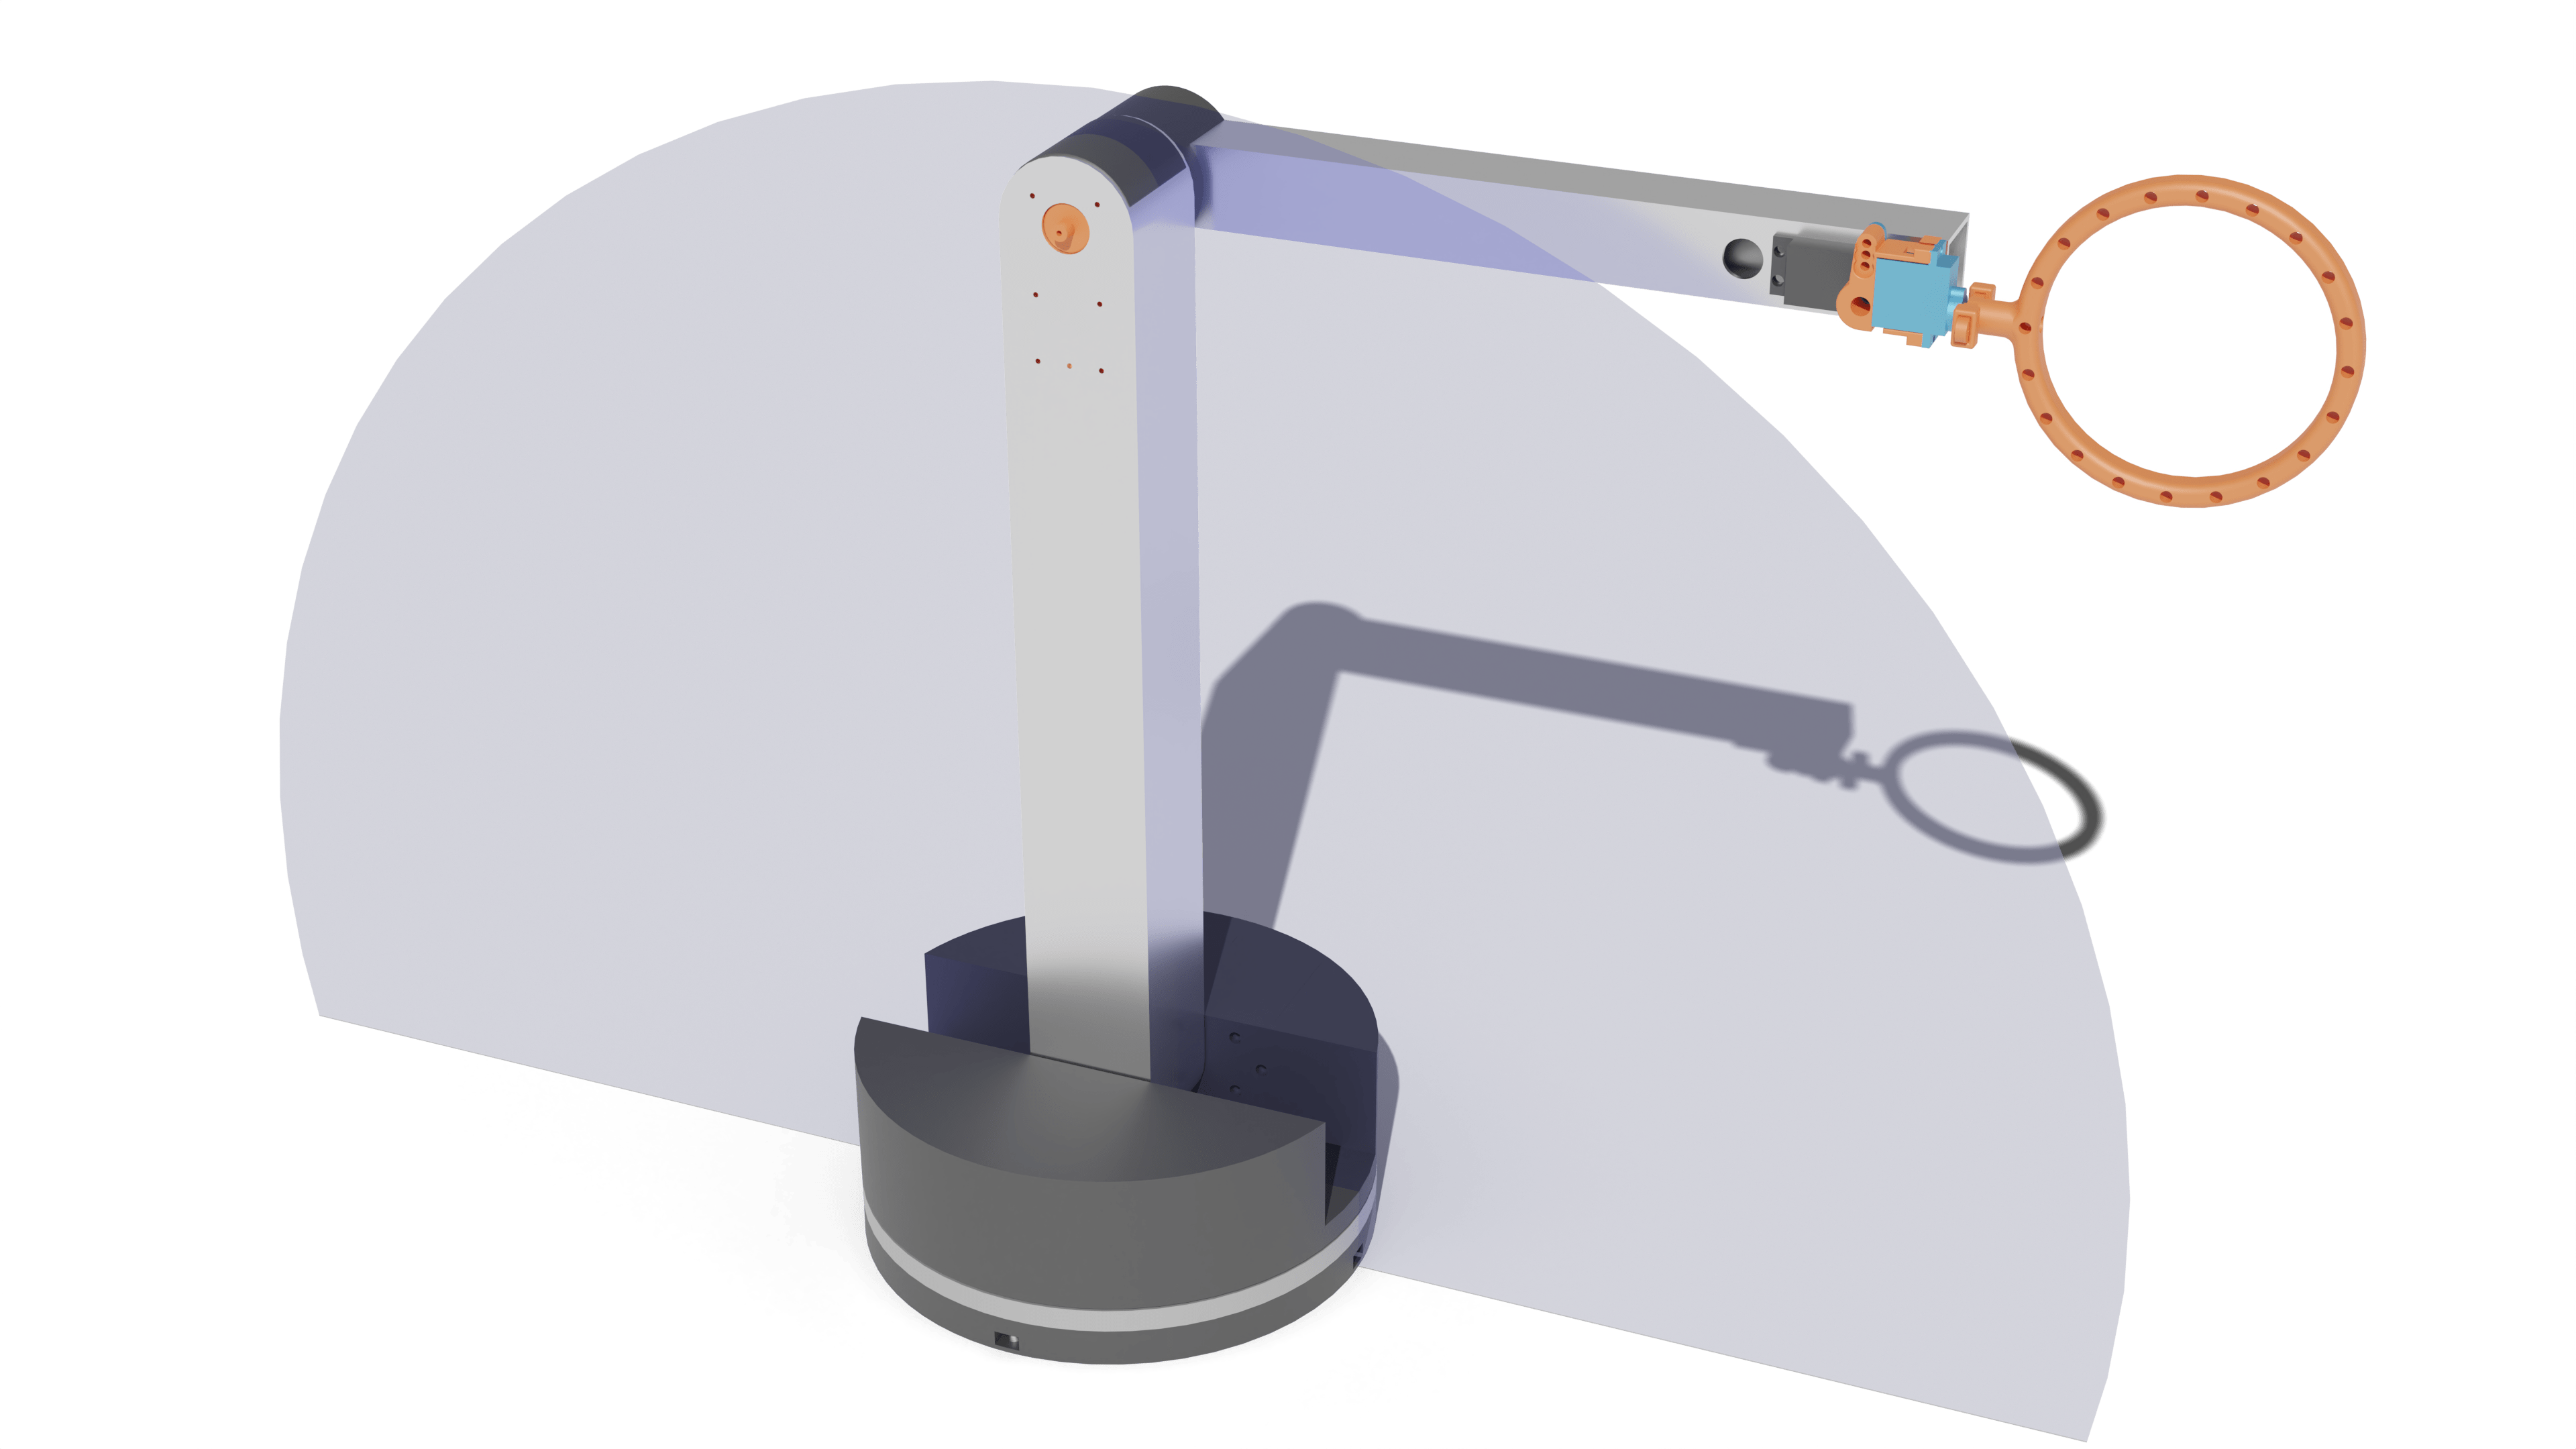
\includegraphics[height = 200pt]{../resources/ArmOnPlane1}
% 	\end{center}
% \end{frame}

% \begin{frame}
% 	\frametitle{Bauspezifikationen}
% 	\begin{center}
% 		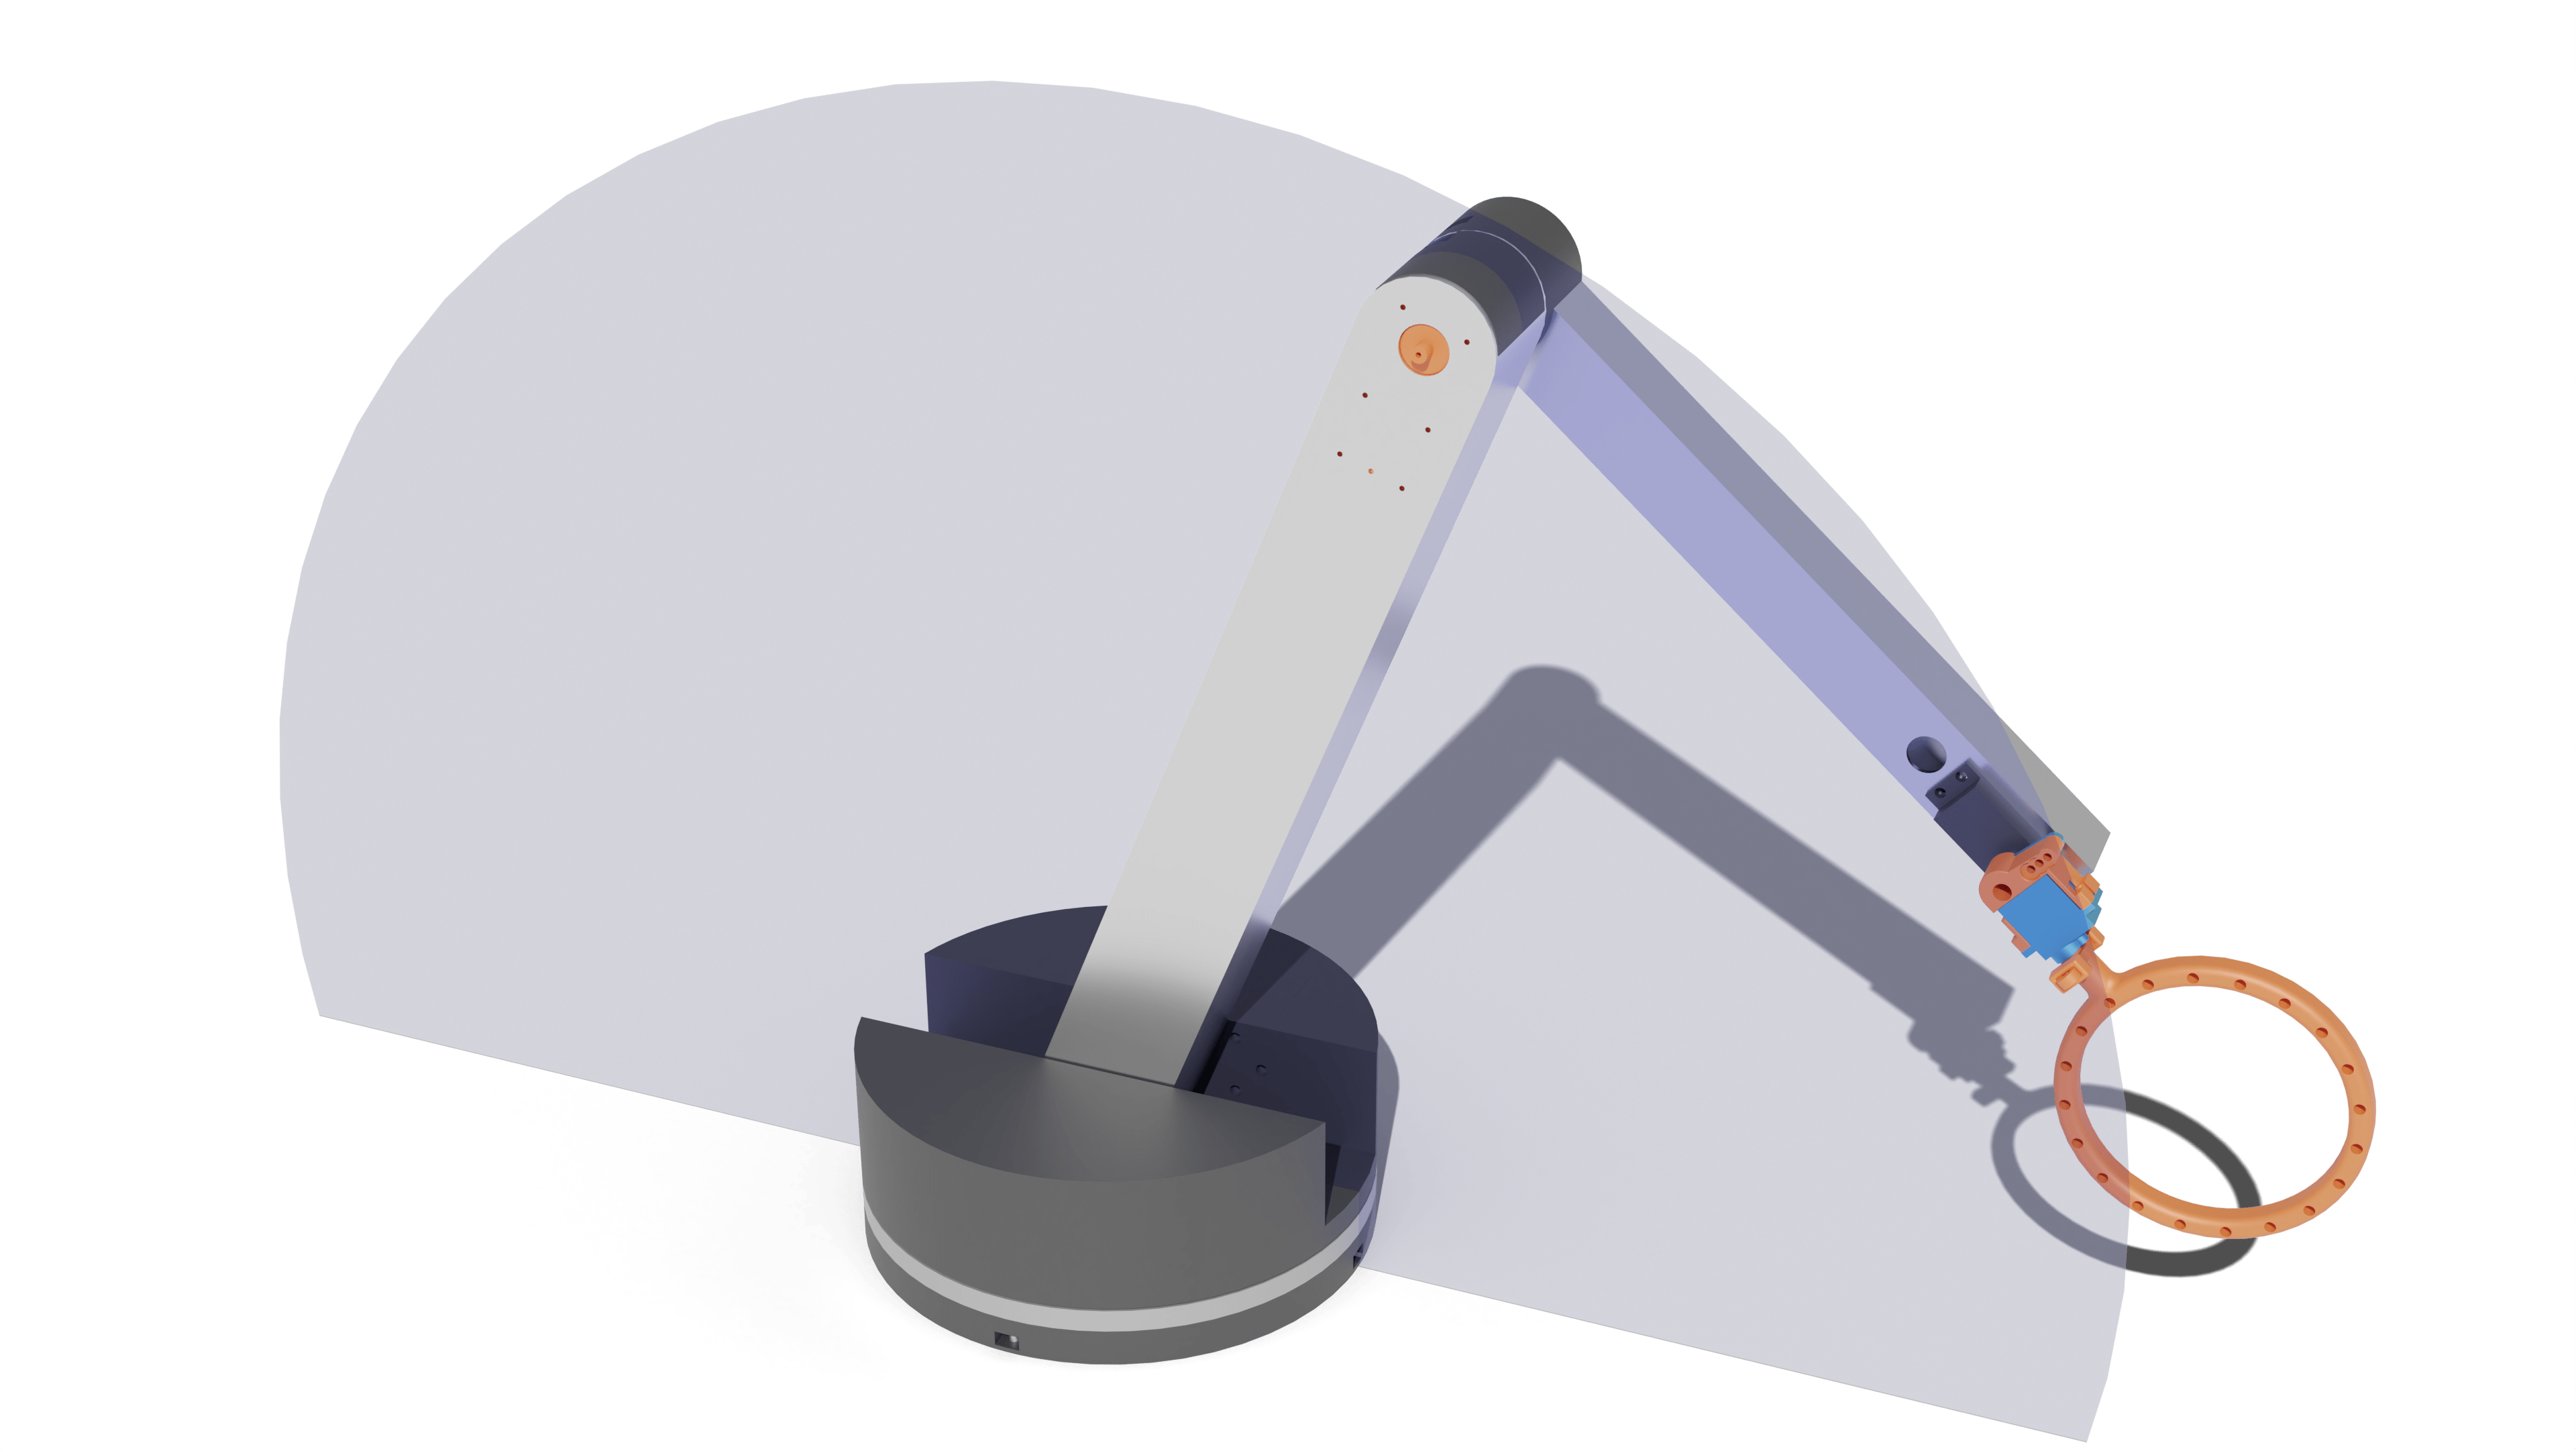
\includegraphics[height = 200pt]{../resources/ArmOnPlane2}
% 	\end{center}
% \end{frame}

% \begin{frame}
% 	\frametitle{Bauspezifikationen}
% 	\begin{center}
% 		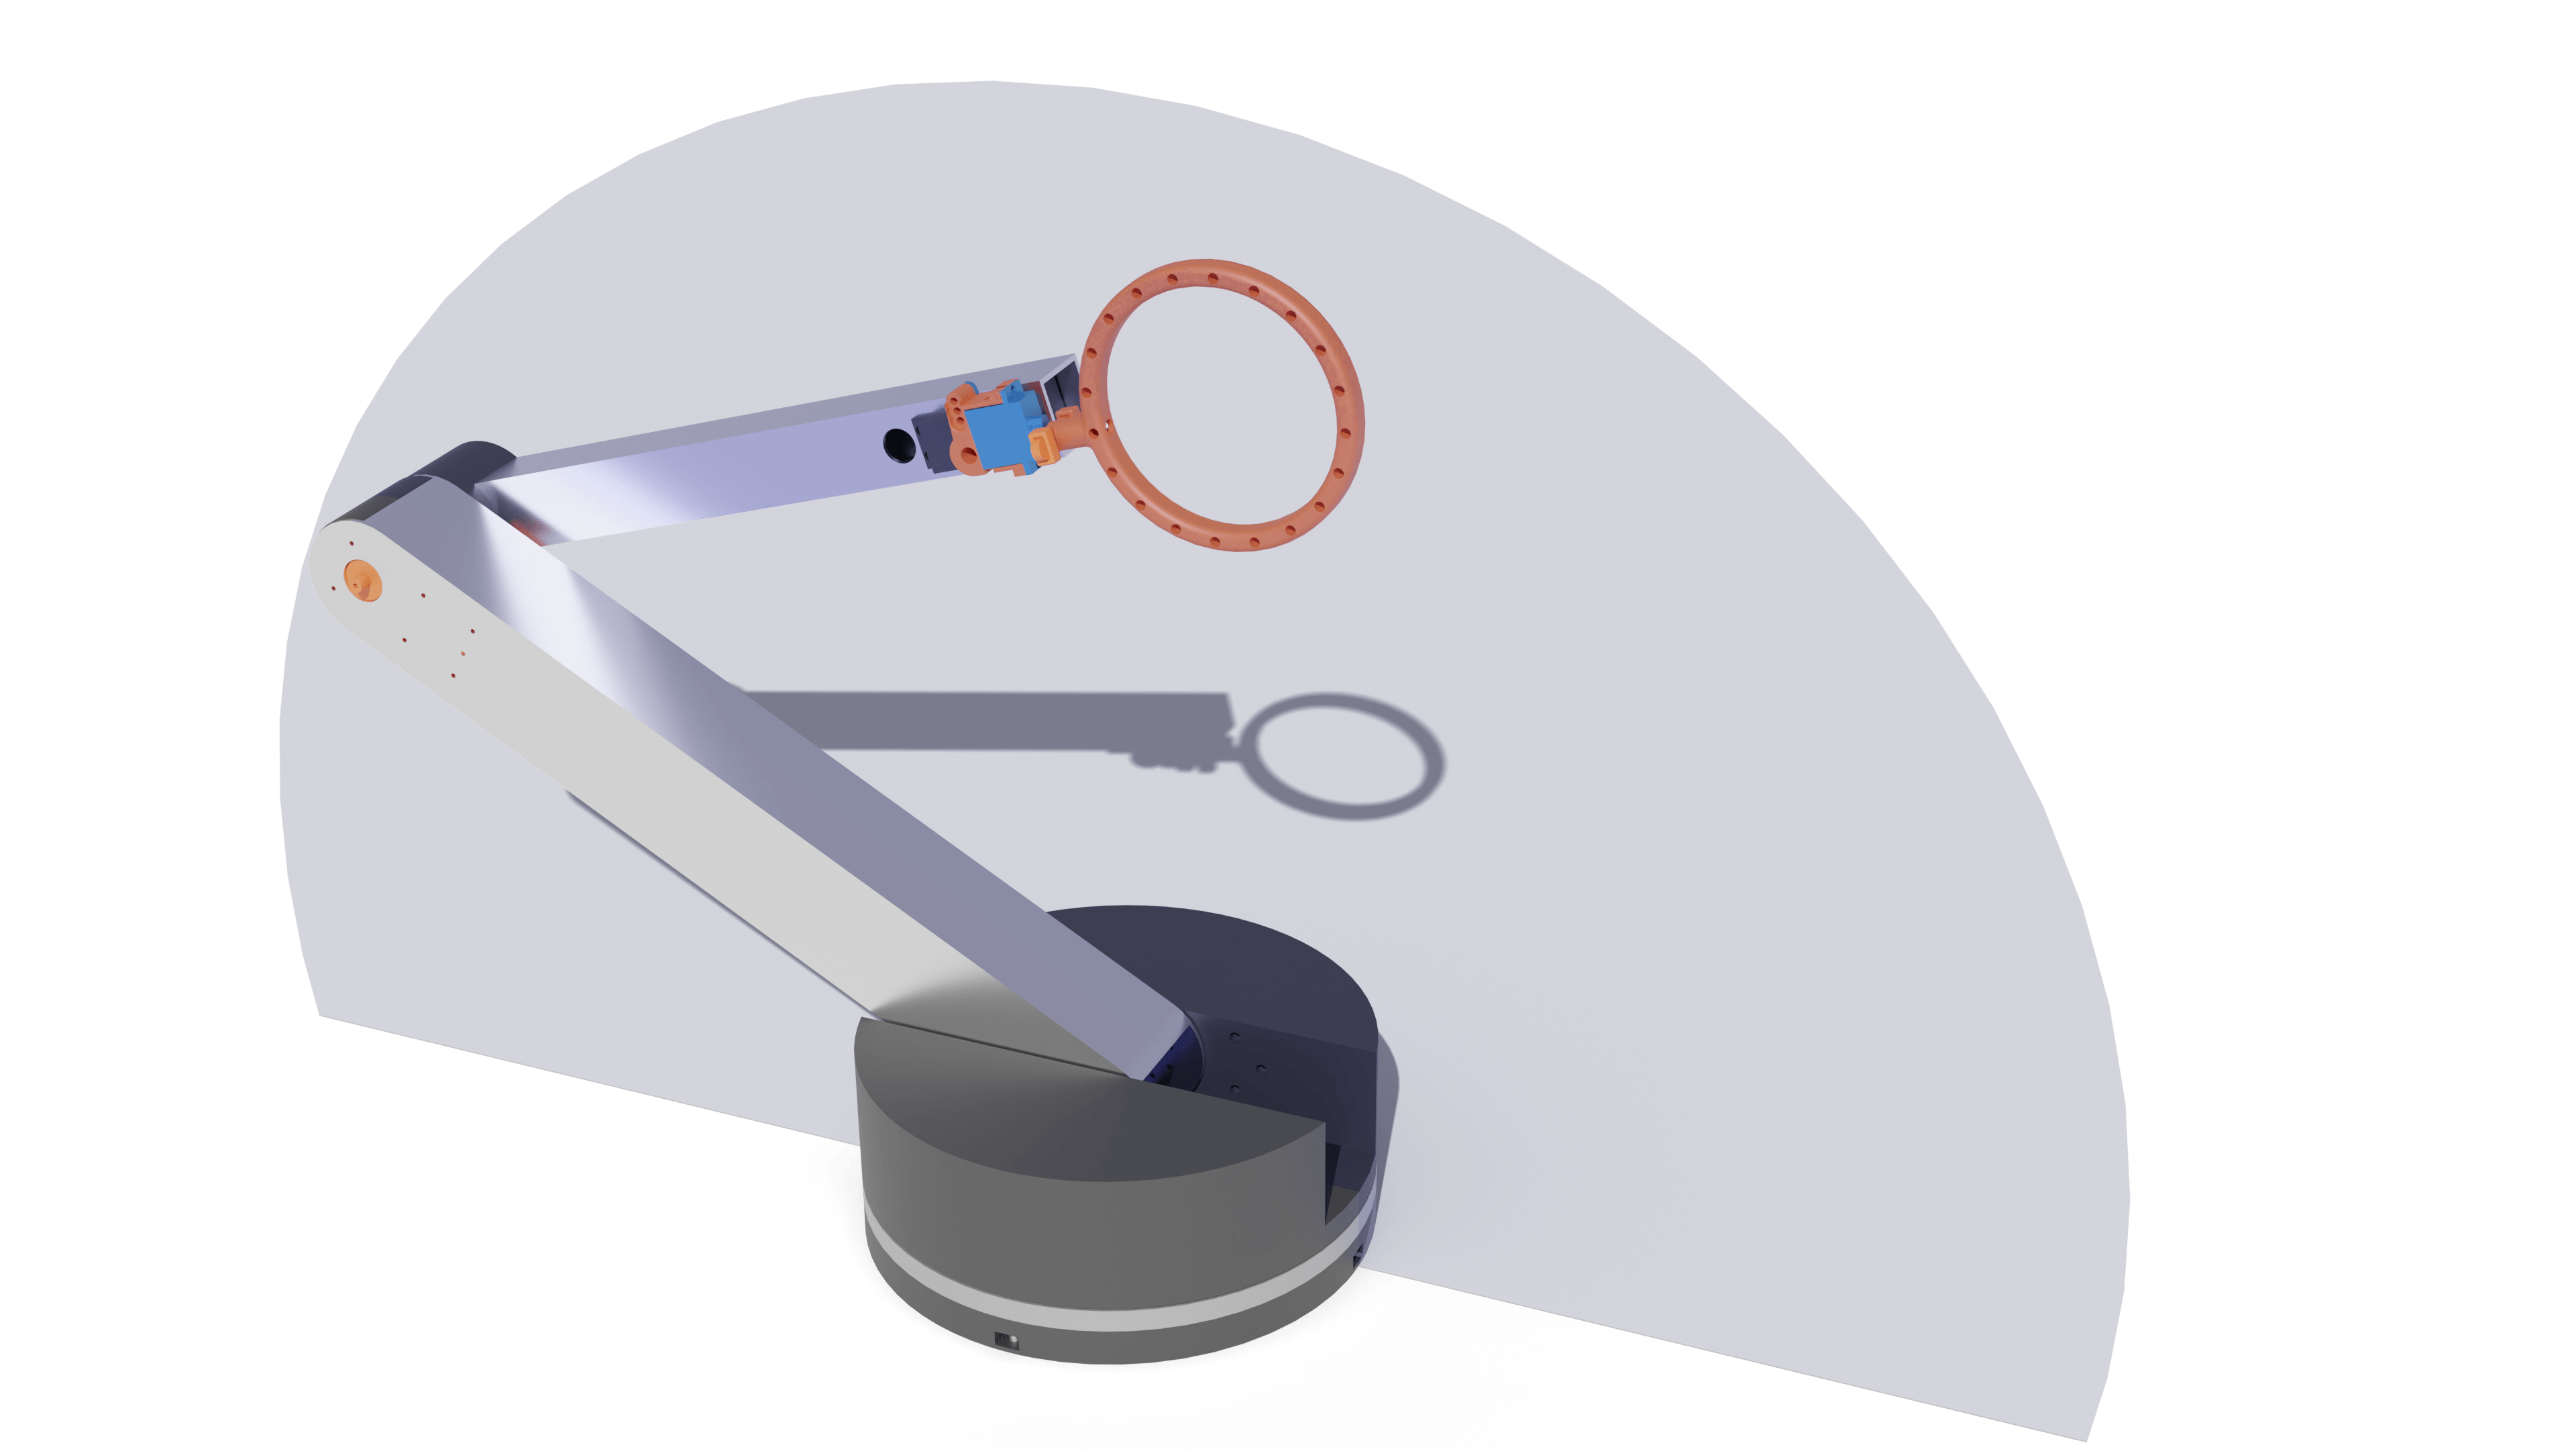
\includegraphics[height = 200pt]{../resources/ArmOnPlane3}
% 	\end{center}
% \end{frame}

% \begin{frame}
% 	\frametitle{Bauspezifikationen}
% 	\begin{center}
% 		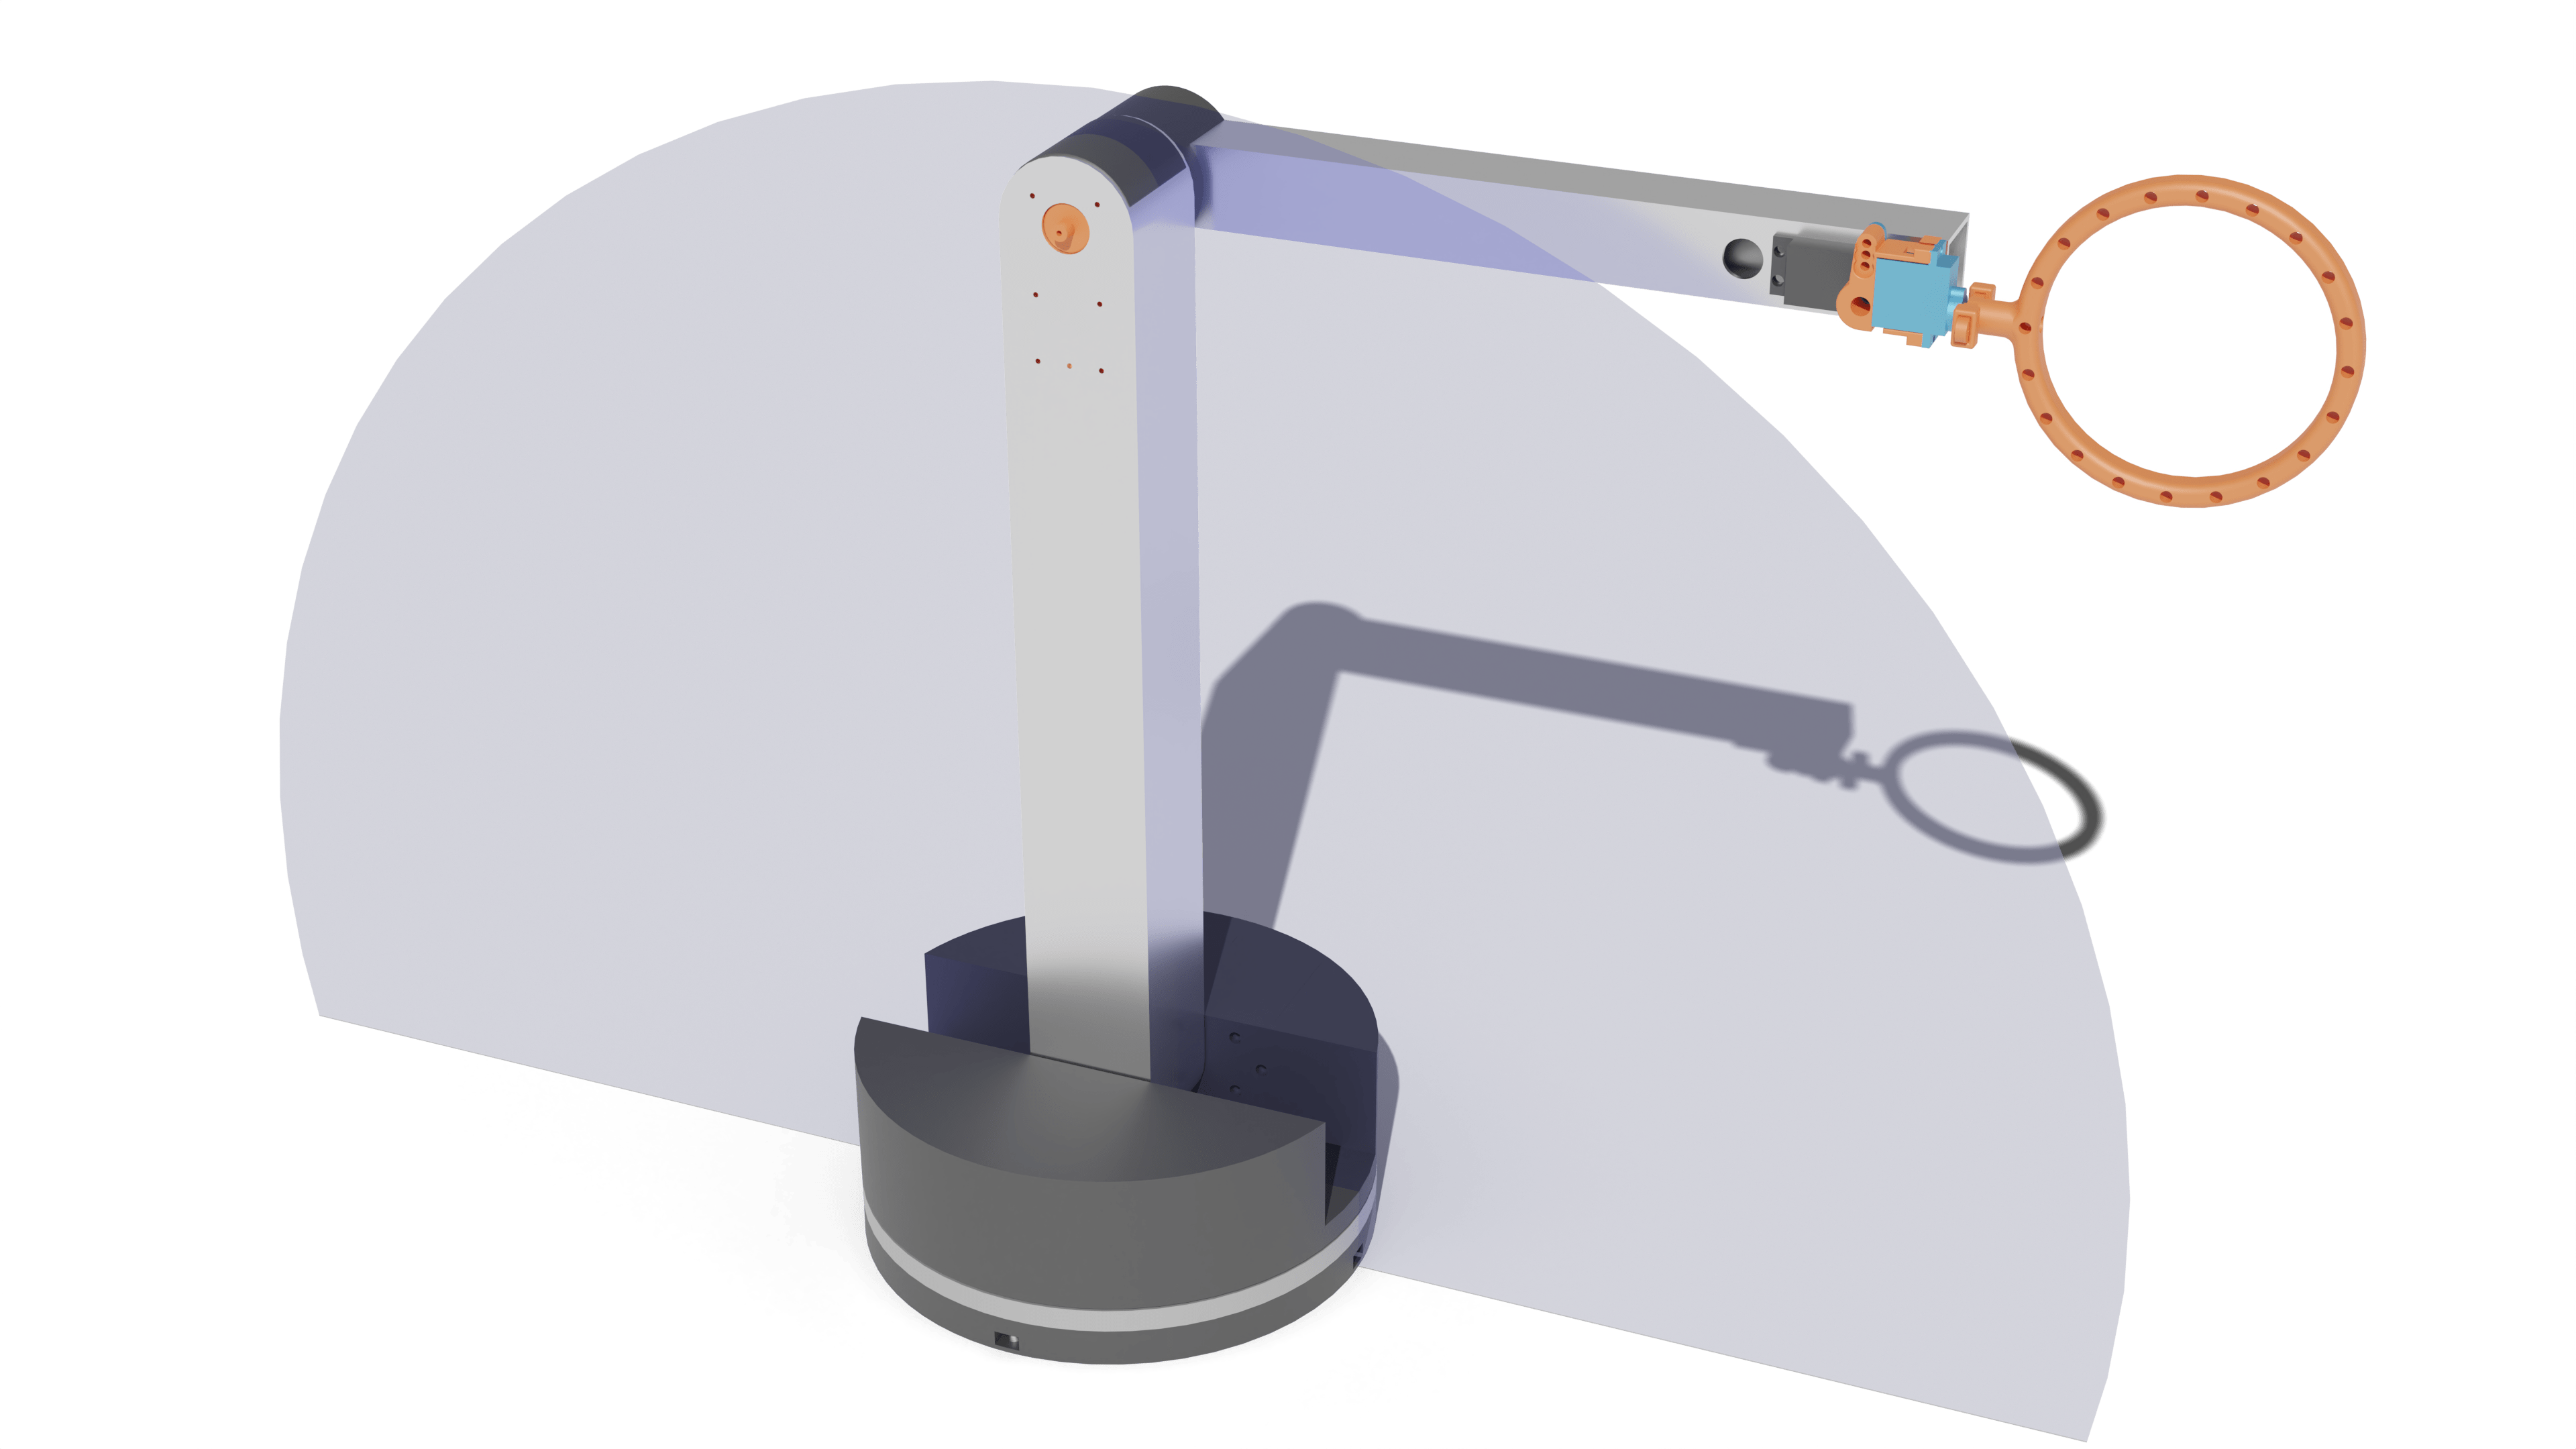
\includegraphics[height = 200pt]{../resources/ArmOnPlane1}
% 	\end{center}
% \end{frame}

\begin{frame}
	\frametitle{Motoren}
	\begin{figure}[h]
		\begin{minipage}[c]{.46\linewidth}
			\centering
			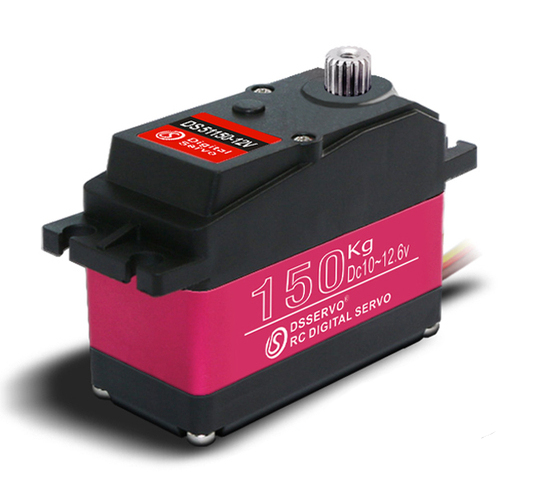
\includegraphics[height = 200pt]{../resources/BaseServo.jpg}
		\end{minipage}
		\hfill%
		\begin{minipage}[c]{.46\linewidth}
			\begin{block}{Basis-Motor}
				\begin{enumerate}
					\item $\omega$ $\approx$ 180 $\frac{deg}{s}$ (Bei 12$\si{\volt}$)
					\item $M$ $\approx$ 15 $\si{\newton}$
					\item Drehbereich: $270^\circ$ ($255^\circ$)
				\end{enumerate}
			\end{block}
		\end{minipage}
	\end{figure}
\end{frame}

\begin{frame}
	\frametitle{Motoren}
	\begin{figure}[h]
		\begin{minipage}[c]{.46\linewidth}
			\centering
			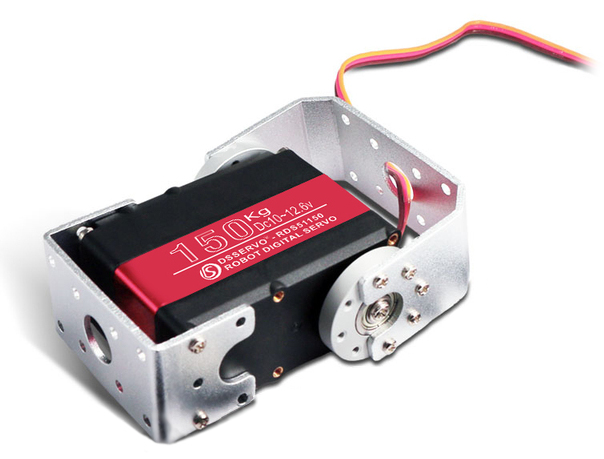
\includegraphics[height = 200pt]{../resources/UpperServo.jpg}
		\end{minipage}
		\hfill%
		\begin{minipage}[c]{.46\linewidth}
			\begin{block}{Arm-Motor}
				\begin{enumerate}
					\item $\omega$ $\approx$ 180 $\frac{deg}{s}$ (Bei 12$\si{\volt}$)
					\item $M$ $\approx$ 15 $\si{\newton}$
					\item Drehbereich: $270^\circ$ ($255^\circ$)
				\end{enumerate}
			\end{block}
		\end{minipage}
	\end{figure}
\end{frame}

% \begin{frame}
% 	\frametitle{Kamerasystem}

% 	\begin{tikzpicture}
% 		\pgfmathsetmacro{\cubex}{2}
% 		\pgfmathsetmacro{\cubey}{1}
% 		\pgfmathsetmacro{\cubez}{1}
% 		\draw[red,fill=yellow] (0,0,0) -- ++(-\cubex,0,0) -- ++(0,-\cubey,0) -- ++(\cubex,0,0) -- cycle;
% 		\draw[red,fill=yellow] (0,0,0) -- ++(0,0,-\cubez) -- ++(0,-\cubey,0) -- ++(0,0,\cubez) -- cycle;
% 		\draw[red,fill=yellow] (0,0,0) -- ++(-\cubex,0,0) -- ++(0,0,-\cubez) -- ++(\cubex,0,0) -- cycle;
% 	\end{tikzpicture}

% \end{frame}


\end{document}
